\documentclass[../main.tex]{subfiles}
\begin{document}
\chapter{Operator \& Ekspresi}

\section*{Tujuan Praktikum}
Setelah menyelesaikan praktikum ini, mahasiswa diharapkan mampu:
\begin{itemize}
  \item Memahami dan menggunakan operator aritmetika (+, -, *, /, div, mod, \%)
  \item Memahami dan menggunakan operator relasional untuk perbandingan
  \item Memahami dan menggunakan operator logika (and, or, not, \&\&, ||, !)
  \item Memahami konsep precedence dan associativity operator
  \item Menulis ekspresi kompleks dengan urutan evaluasi yang benar
  \item Menggunakan tanda kurung untuk memperjelas dan mengubah urutan evaluasi
\end{itemize}

\section{Operator Aritmetika, Relasional, Logika}
Operator-operator fundamental dalam pemrograman terbagi menjadi tiga kategori utama: aritmetika (mencakup \texttt{+}, \texttt{-}, \texttt{*}, operasi pembagian, dan sisa bagi), relasional (seperti \texttt{\textless}, \texttt{\textless=}, \texttt{==} atau \texttt{=}, \texttt{\textgreater}, \texttt{\textgreater=}), serta logika (\texttt{and}/\texttt{or}/\texttt{not} di Pascal, atau \texttt{\&\&}/\texttt{||}/\texttt{!} di C/C++). Ketiga jenis operator ini menjadi fondasi dalam evaluasi ekspresi. Penting untuk memperhatikan perbedaan antara pembagian integer dan floating-point, serta konvensi operator equality yang berbeda antar bahasa \parencite{pascal-tutorial-wikibooks,gnu-c-manual,cpp-reference}.

Untuk ekspresi yang panjang dan kompleks, sebaiknya gunakan tanda kurung secara eksplisit untuk memperjelas maksud Anda. Jangan ragu memecah ekspresi yang rumit menjadi beberapa variabel intermediate dengan nama yang deskriptif—ini akan memudahkan testing dan debugging. Untuk detail lengkap mengenai prioritas dan asosiativitas operator, rujuklah tabel resmi yang tersedia di dokumentasi masing-masing bahasa \parencite{gnu-c-manual,cpp-op-precedence,c-op-precedence}.

\subsection{Ringkasan Operator Umum}
\begin{table}[H]
  \centering
  \caption{Operator umum lintas bahasa (ringkas)}
  \begin{tabular}{@{}llll@{}}
    \toprule
    Kategori & Pascal & C & C++ \\
    \midrule
    Aritmetika & \texttt{+ - * / div mod} & \texttt{+ - * / \%} & \texttt{+ - * / \%} \\
    Relasional & \texttt{= {\textless}{\textgreater} {\textless} {\textless}= {\textgreater} {\textgreater}=} & \texttt{== != {\textless} {\textless}= {\textgreater} {\textgreater}=} & sama dengan C \\
    Logika & \texttt{and or not} & \texttt{\&\& || !} & sama dengan C \\
    Penugasan & \texttt{:=} & \texttt{=} & \texttt{=} \\
    Inkremen & (tidak ada) & \texttt{++ --} & \texttt{++ --} \\
    \bottomrule
  \end{tabular}
\end{table}

\subsection{Operator Bitwise (C/C++)}
Operator bitwise melakukan operasi langsung pada level bit dalam representasi biner angka. Kategori ini meliputi: AND bit (\texttt{\&}), OR bit (\texttt{|}), XOR (\texttt{\^{}}), NOT bit (\texttt{\textasciitilde}), dan shift operations baik ke kiri maupun kanan (\texttt{<<}, \texttt{>>}). Operator-operator ini sangat bermanfaat untuk bit masking, manipulasi flag, dan berbagai operasi low-level programming \parencite{c-bitwise-ops,cpp-bitwise-ops}.

\begin{lstlisting}[language=C, caption={Contoh operator bitwise di C}]
#include <stdio.h>
int main(void) {
  unsigned x = 0b0101;   // 5
  unsigned y = 0b0011;   // 3
  printf("x & y = %u\n", x & y);  // 1
  printf("x | y = %u\n", x | y);  // 7
  printf("x ^ y = %u\n", x ^ y);  // 6
  printf("~x    = %u\n", (unsigned)~x);
  printf("x << 1 = %u\n", x << 1); // 10
  printf("x >> 1 = %u\n", x >> 1); // 2
}
\end{lstlisting}

\subsection{Short-Circuit dan Operator Kondisional}
Di C dan C++, operator logika \texttt{\&\&} serta \texttt{||} mengimplementasikan mekanisme short-circuit evaluation—artinya, operand di sisi kanan tidak akan dievaluasi apabila hasil akhir sudah dapat ditentukan dari operand kiri saja. Selain itu, terdapat operator kondisional ternary (\texttt{?:}) yang berfungsi memilih satu dari dua ekspresi berdasarkan evaluasi kondisi boolean. Pemahaman mengenai konsep ini akan menjadi lebih solid setelah Anda mempelajari struktur percabangan pada bab berikutnya \parencite{c-conditional-operator,cpp-conditional-operator}.

\subsection{Contoh Operator Aritmetika}

Program-program berikut mengilustrasikan penggunaan seluruh operator aritmetika dasar. Perhatikan khususnya perbedaan antara pembagian real (\texttt{/}) yang menghasilkan desimal dengan pembagian integer (\texttt{div}):

\begin{lstlisting}[language=Pascal, caption={Operator aritmetika di Pascal}]
program OperatorAritmatika;
var
  a, b: integer;
begin
  a := 10;
  b := 3;
  Writeln('Penjumlahan: ', a + b);
  Writeln('Pengurangan: ', a - b);
  Writeln('Perkalian: ', a * b);
  Writeln('Pembagian real: ', a / b:0:2);
  Writeln('Pembagian bulat: ', a div b);
  Writeln('Modulus: ', a mod b);
end.
\end{lstlisting}

Implementasi yang sama dalam bahasa C, dengan perhatian khusus pada teknik type casting yang diperlukan untuk pembagian real:

\begin{lstlisting}[language=C, caption={Operator aritmetika di C}]
#include <stdio.h>
int main(void) {
  int a = 10, b = 3;
  printf("Penjumlahan: %d\n", a + b);
  printf("Pengurangan: %d\n", a - b);
  printf("Perkalian: %d\n", a * b);
  printf("Pembagian real: %.2f\n", (float)a / b);
  printf("Pembagian bulat: %d\n", a / b);
  printf("Modulus: %d\n", a % b);
  return 0;
}
\end{lstlisting}

Dalam C++, sintaksnya terlihat sedikit lebih modern meski logic-nya tetap identik:

\begin{lstlisting}[language=C++, caption={Operator aritmetika di C++}]
#include <iostream>
using namespace std;

int main() {
  int a = 10, b = 3;
  cout << "Penjumlahan: " << a + b << "\n";
  cout << "Pengurangan: " << a - b << "\n";
  cout << "Perkalian: " << a * b << "\n";
  cout << "Pembagian real: " << (float)a / b << "\n";
  cout << "Pembagian bulat: " << a / b << "\n";
  cout << "Modulus: " << a % b << "\n";
}
\end{lstlisting}

\subsection{Contoh Operator Relasional dan Logika}

Contoh-contoh berikut memperlihatkan bagaimana operator perbandingan dan operator logika digunakan untuk menyusun ekspresi boolean yang lebih kompleks:

\begin{lstlisting}[language=Pascal, caption={Operator relasional dan logika di Pascal}]
program OperatorRelasionalLogika;
var
  a, b: integer;
  hasil: boolean;
begin
  a := 10;
  b := 5;
  { Operator Relasional }
  hasil := a > b;
  Writeln('a > b: ', hasil);
  hasil := a = b;
  Writeln('a = b: ', hasil);
  hasil := a <> b;
  Writeln('a <> b: ', hasil);
  { Operator Logika }
  hasil := (a > b) and (b > 0);
  Writeln('(a > b) and (b > 0): ', hasil);
  hasil := (a < b) or (b > 0);
  Writeln('(a < b) or (b > 0): ', hasil);
  hasil := not (a = b);
  Writeln('not (a = b): ', hasil);
end.
\end{lstlisting}

Dalam bahasa C, operator relasional dan logika menghasilkan nilai integer—dimana 0 merepresentasikan false dan nilai non-zero merepresentasikan true:

\begin{lstlisting}[language=C, caption={Operator relasional dan logika di C}]
#include <stdio.h>
int main(void) {
  int a = 10, b = 5;
  int hasil;
  // Operator Relasional
  hasil = a > b;
  printf("a > b: %d\n", hasil);
  hasil = a == b;
  printf("a == b: %d\n", hasil);
  hasil = a != b;
  printf("a != b: %d\n", hasil);
  // Operator Logika
  hasil = (a > b) && (b > 0);
  printf("(a > b) && (b > 0): %d\n", hasil);
  hasil = (a < b) || (b > 0);
  printf("(a < b) || (b > 0): %d\n", hasil);
  hasil = !(a == b);
  printf("!(a == b): %d\n", hasil);
  return 0;
}
\end{lstlisting}

C++ menyediakan tipe data \texttt{bool} yang lebih eksplisit dan type-safe untuk merepresentasikan nilai boolean:

\begin{lstlisting}[language=C++, caption={Operator relasional dan logika di C++}]
#include <iostream>
using namespace std;

int main() {
  int a = 10, b = 5;
  bool hasil;
  // Operator Relasional
  hasil = a > b;
  cout << "a > b: " << hasil << "\n";
  hasil = a == b;
  cout << "a == b: " << hasil << "\n";
  hasil = a != b;
  cout << "a != b: " << hasil << "\n";
  // Operator Logika
  hasil = (a > b) && (b > 0);
  cout << "(a > b) && (b > 0): " << hasil << "\n";
  hasil = (a < b) || (b > 0);
  cout << "(a < b) || (b > 0): " << hasil << "\n";
  hasil = !(a == b);
  cout << "!(a == b): " << hasil << "\n";
}
\end{lstlisting}

\section{Precedence vs Order of Evaluation}
Precedence dan associativity mengatur cara suatu ekspresi di-grouping tanpa perlu tanda kurung eksplisit. Namun, order of evaluation (urutan aktual ketika operand dievaluasi) adalah konsep yang berbeda dan terpisah. Di C/C++, sejumlah operator tidak menjamin urutan evaluasi operand-nya, sehingga jika ada side effect yang berulang pada variabel yang sama, hal ini bisa memicu undefined behavior. Untuk menghindari masalah tersebut, selalu gunakan parentheses dan pecah ekspresi kompleks ke dalam variabel perantara \parencite{gnu-c-manual,cpp-op-precedence,c-op-precedence,c-order-of-eval,cpp-order-of-eval}.

\subsection{Penjelasan Precedence dan Associativity}
Precedence (atau prioritas operator) menentukan operator mana yang akan dieksekusi lebih dulu dalam sebuah ekspresi yang tidak menggunakan kurung. Operator yang memiliki precedence lebih tinggi akan diproses terlebih dahulu dibanding operator dengan precedence rendah. Di sisi lain, associativity (asosiativitas) menentukan arah evaluasi ketika ada beberapa operator dengan tingkat precedence yang sama—apakah dari kiri ke kanan, atau dari kanan ke kiri.

Agar urutan evaluasi dalam ekspresi yang kompleks benar-benar sesuai dengan yang diinginkan, biasakan untuk menambahkan tanda kurung secara eksplisit. Pendekatan ini tidak hanya meningkatkan readability, tetapi juga mencegah bug logika yang seringkali sulit di-trace.

\subsection{Tabel Precedence Operator}
\begin{table}[H]
  \centering
  \caption{Precedence operator (tinggi ke rendah)}
  \begin{tabular}{@{}llll@{}}
    \toprule
    Level & Operator & Associativity & Kategori \\
    \midrule
    1 & \texttt{()}, \texttt{[]} & kiri-ke-kanan & Pengelompokan, array \\
    2 & \texttt{++}, \texttt{--} (postfix) & kiri-ke-kanan & Increment/decrement \\
    3 & \texttt{!}, \texttt{not}, unary \texttt{+}, \texttt{-} & kanan-ke-kiri & Unary \\
    4 & \texttt{*}, \texttt{/}, \texttt{\%}, \texttt{mod}, \texttt{div} & kiri-ke-kanan & Multiplikatif \\
    5 & \texttt{+}, \texttt{-} & kiri-ke-kanan & Additif \\
    6 & \texttt{<}, \texttt{<=}, \texttt{>}, \texttt{>=} & kiri-ke-kanan & Relasional \\
    7 & \texttt{==}, \texttt{!=}, \texttt{=}, \texttt{<>} & kiri-ke-kanan & Kesetaraan \\
    8 & \texttt{\&\&}, \texttt{and} & kiri-ke-kanan & Logika AND \\
    9 & \texttt{||}, \texttt{or} & kiri-ke-kanan & Logika OR \\
    10 & \texttt{=}, \texttt{:=}, \texttt{+=}, \texttt{-=} & kanan-ke-kiri & Penugasan \\
    \bottomrule
  \end{tabular}
  \\Sumber: \parencite{gnu-c-manual,cpp-op-precedence,c-op-precedence}
\end{table}

\subsection{Sketsa Pohon Ekspresi}
Untuk mempermudah pemahaman tentang bagaimana precedence bekerja, mari kita lihat representasi pohon ekspresi berikut. Pohon ini menggambarkan urutan evaluasi, dimana operator di level bawah (prioritas tinggi) dievaluasi terlebih dahulu, baru kemudian naik ke atas (prioritas rendah):

\begin{figure}[H]
  \centering
  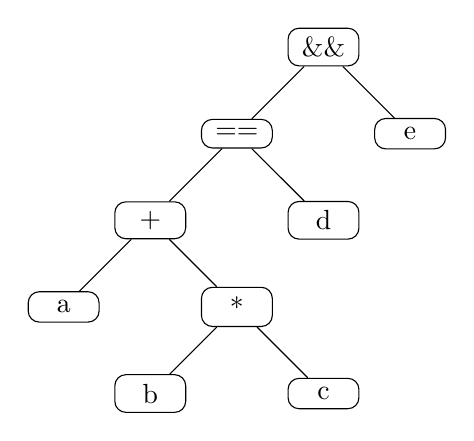
\begin{tikzpicture}[level distance=1.1cm, sibling distance=2.2cm]
    \tikzstyle{n}=[draw, rounded corners, minimum width=9mm, align=center]
    \node[n]{\&\&}
      child{ node[n]{==}
        child{ node[n]{+}
          child{ node[n]{a} }
          child{ node[n]{*}
            child{ node[n]{b} }
            child{ node[n]{c} }
          }
        }
        child{ node[n]{d} }
      }
      child{ node[n]{e} };
  \end{tikzpicture}
  \caption{Precedence: \texttt{*} \textgreater{} \texttt{+} \textgreater{} \texttt{==} \textgreater{} \texttt{\&\&}}
\end{figure}

Dalam visualisasi pohon tersebut, operator \texttt{*} (multiplication) menempati posisi paling bawah—ini berarti ia dievaluasi paling awal. Setelahnya, evaluasi berlanjut ke operator \texttt{+}, kemudian \texttt{==}, dan akhirnya operator \texttt{\&\&} di puncak pohon. Struktur ini merepresentasikan ekspresi: \texttt{(a + b * c) == d \&\& e}.

\subsection{Contoh Demonstrasi Precedence}

Contoh-contoh program berikut memperlihatkan secara konkret bagaimana precedence operator mempengaruhi hasil evaluasi ekspresi, serta bagaimana penggunaan tanda kurung dapat mengubah urutan evaluasi dan hasil akhir:

\begin{lstlisting}[language=Pascal, caption={Precedence operator di Pascal}]
program PrecedenceDemo;
var
  a, b, c, hasil: integer;
begin
  a := 10;
  b := 5;
  c := 2;
  { Perkalian (*) memiliki precedence lebih tinggi dari penjumlahan (+) }
  hasil := a + b * c;
  Writeln('a + b * c = ', hasil);        { Output: 20 }
  Writeln('(a + b) * c = ', (a + b) * c); { Output: 30 }
  
  { Operator dengan precedence sama: evaluasi kiri-ke-kanan }
  hasil := a - b + c;
  Writeln('a - b + c = ', hasil);        { Output: 7 }
  Writeln('a - (b + c) = ', a - (b + c)); { Output: 3 }
end.
\end{lstlisting}

Implementasi dalam C mengilustrasikan prinsip yang sama, ditambah dengan contoh penggunaan operator relasional dan logika:

\begin{lstlisting}[language=C, caption={Precedence operator di C}]
#include <stdio.h>
int main(void) {
  int a = 10, b = 5, c = 2;
  int hasil;
  // Perkalian (*) memiliki precedence lebih tinggi dari penjumlahan (+)
  hasil = a + b * c;
  printf("a + b * c = %d\n", hasil);        // Output: 20
  printf("(a + b) * c = %d\n", (a + b) * c); // Output: 30
  
  // Operator dengan precedence sama: evaluasi kiri-ke-kanan
  hasil = a - b + c;
  printf("a - b + c = %d\n", hasil);        // Output: 7
  printf("a - (b + c) = %d\n", a - (b + c)); // Output: 3
  
  // Operator relasional dan logika
  hasil = a > b && b > c;
  printf("(a > b) && (b > c) = %d\n", hasil); // Output: 1 (true)
  return 0;
}
\end{lstlisting}

Dalam C++, kita menggunakan tipe boolean eksplisit untuk mendemonstrasikan operator logika dengan lebih jelas:

\begin{lstlisting}[language=C++, caption={Precedence operator di C++}]
#include <iostream>
using namespace std;

int main() {
  int a = 10, b = 5, c = 2;
  int hasil;
  // Perkalian (*) memiliki precedence lebih tinggi dari penjumlahan (+)
  hasil = a + b * c;
  cout << "a + b * c = " << hasil << "\n";        // Output: 20
  cout << "(a + b) * c = " << (a + b) * c << "\n"; // Output: 30
  
  // Operator dengan precedence sama: evaluasi kiri-ke-kanan
  hasil = a - b + c;
  cout << "a - b + c = " << hasil << "\n";        // Output: 7
  cout << "a - (b + c) = " << a - (b + c) << "\n"; // Output: 3
  
  // Operator relasional dan logika
  bool cek = (a > b) && (b > c);
  cout << "(a > b) && (b > c) = " << cek << "\n"; // Output: 1 (true)
}
\end{lstlisting}

Contoh-contoh di atas menggambarkan dengan jelas bagaimana precedence berpengaruh terhadap hasil akhir evaluasi. Ketika kita menulis \texttt{a + b * c} tanpa kurung, ekspresi tersebut diperlakukan sebagai \texttt{a + (b * c)} karena multiplication memiliki precedence yang lebih tinggi dibanding addition. Namun, jika kita menambahkan tanda kurung eksplisit seperti \texttt{(a + b) * c}, maka urutan evaluasinya berubah total dan tentu saja menghasilkan nilai yang berbeda pula.

\section{Perilaku Tak Terdefinisi: Contoh Klasik}
Sangat penting untuk menghindari ekspresi yang melakukan side effect berulang kali pada objek atau variabel yang sama tanpa ada sequence point yang memisahkan operasi-operasi tersebut dengan jelas.

Program berikut menunjukkan sebuah contoh klasik dari undefined behavior—dimana variabel yang sama dimodifikasi dan digunakan beberapa kali dalam satu ekspresi:

\begin{lstlisting}[language=C, caption={Contoh UB: increment dan penggunaan berulang}]
#include <stdio.h>
int main(void) {
  int i = 1;
  int a = i++ + i++; // tak terdefinisi di C: jangan lakukan ini
  printf("%d\n", a);
}
\end{lstlisting}

Untuk menghindari masalah tersebut, pisahkan setiap langkah operasi agar portable dan mudah dipahami. Berikut adalah pendekatan yang aman untuk melakukan operasi serupa:

\begin{lstlisting}[language=C]
int i = 1;
int a = i;
int b = i + 1;
i += 2;
int sum = a + b; // aman dan jelas
\end{lstlisting}

\section{Rangkuman Materi}
\begin{itemize}
  \item Kita telah membahas berbagai jenis operator—mulai dari aritmetika, relasional, logika, hingga bitwise—yang tersedia di ketiga bahasa pemrograman.
  \item Mekanisme short-circuit evaluation pada operator \texttt{\&\&} dan \texttt{||}, serta penggunaan operator ternary untuk conditional expression, telah dijelaskan dengan contoh.
  \item Perbedaan penting antara \emph{precedence/associativity} (yang menentukan grouping) dan \emph{order of evaluation} (urutan aktual eksekusi operand) telah diuraikan, termasuk konsekuensi dari side effect yang tidak aman.
  \item Contoh-contoh kode yang menimbulkan undefined behavior (UB) telah ditunjukkan, beserta pattern yang aman menggunakan variabel perantara untuk memisahkan setiap operasi.
  \item Tabel precedence operator dan diagram pohon ekspresi disertakan untuk membantu visualisasi bagaimana ekspresi di-grouping dan dievaluasi.
\end{itemize}

\end{document}
